
\chapter{Réalisation}
    \section{Électronique}
    % mettre analyse SysML et Schéma électronique cote à cote
    
    Le schéma structurel et le routage de la carte ont été effectués avec le logiciel en ligne UpVerter\footnote{Schéma : \href{https://upverter.com/OrboxTeam/cfa40d292bac9e7b/Orbox_PFE/}{OrBox PFE - upverter.com} --- Nomenclature : \href{https://docs.google.com/spreadsheets/d/1U8SqlsJ5GUVQXFXz04T_kTUTFbFambgKo4qdCGi8VkM/edit?usp=sharing}{BOM - docs.google.com}}. Cette section donne des précisions sur la manière dont chaque fonction électronique a été implémentée. 
        
\begin{figure}[H]
    \centerline{
        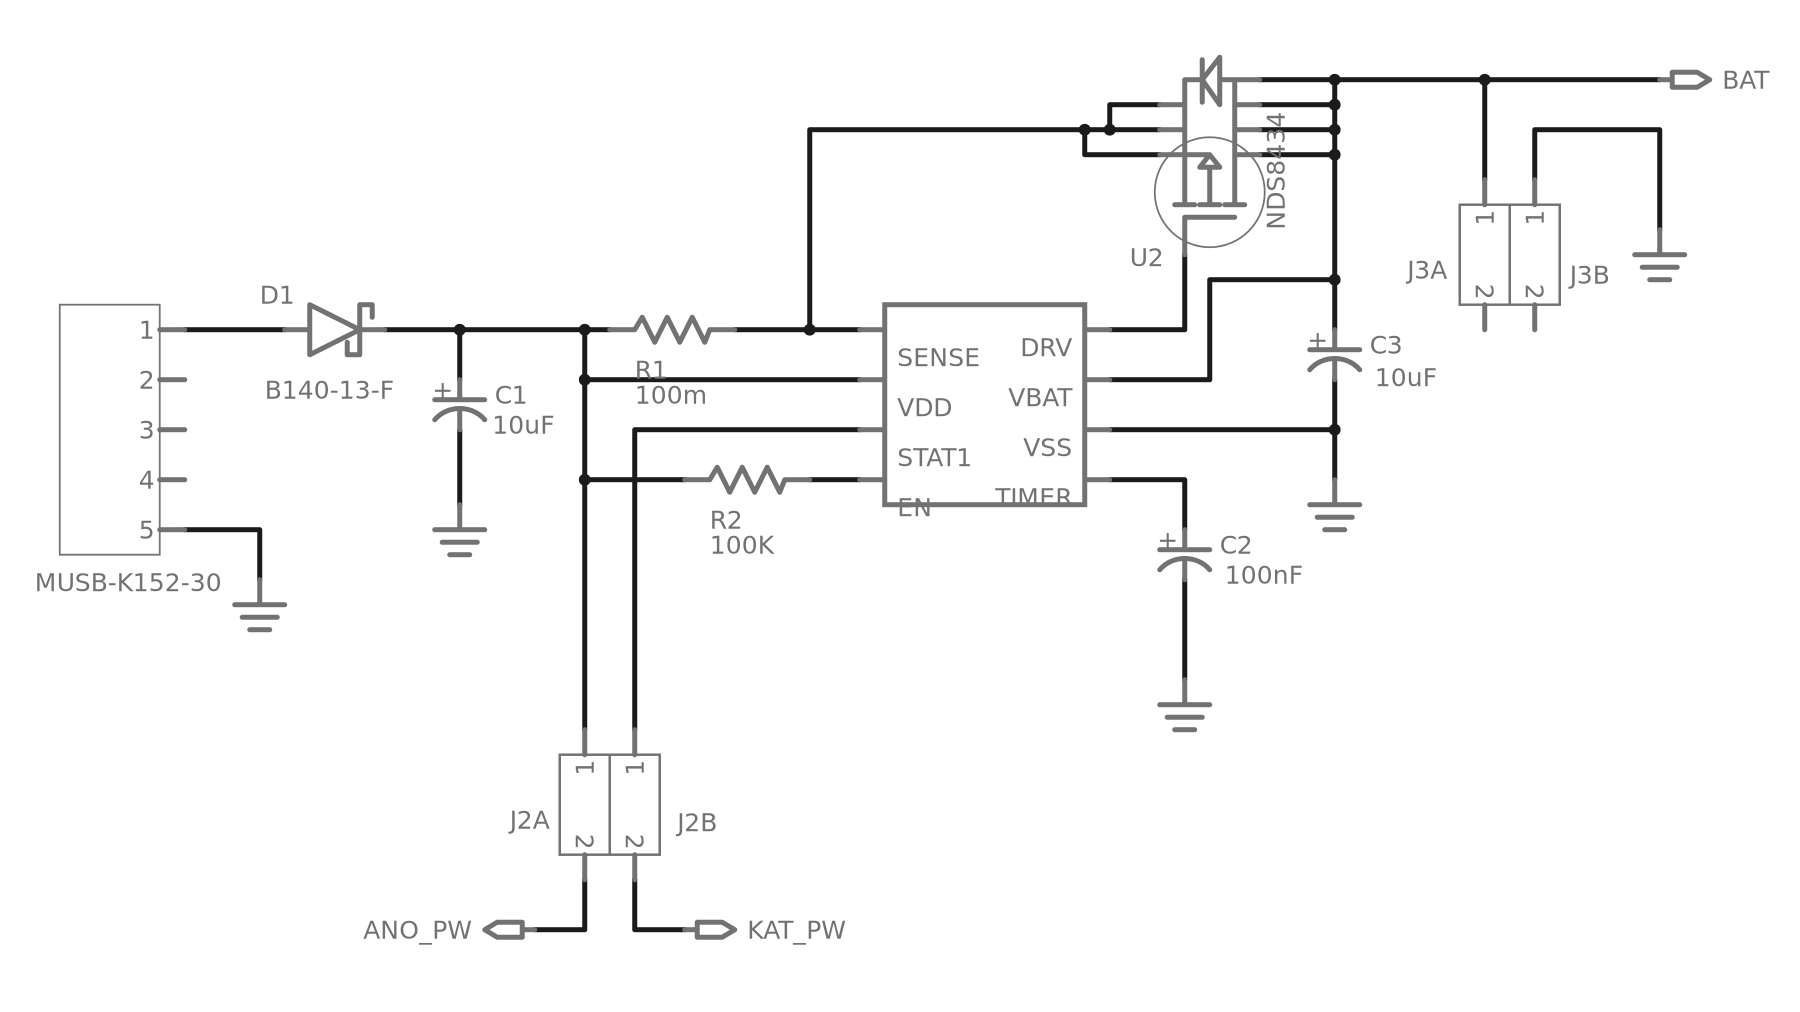
\includegraphics[width=0.85\textwidth,fbox]{img/ElecSch_BatCharger}
    }
    \caption{Schéma structurel du régulateur de charge}
    \label{ElecSch_BatCharger}
\end{figure}

    La fonction électronique \emph{régulateur de charge} est réalisée autour du composant MCP73843 (repère typographique $U_1$ de la Figure \ref{ElecSch_BatCharger}).
    Pour rappel, la fonction régulateur de charge a pour rôle de prendre la tension d'entrée de 5V délivrée par le chargeur USB mural pour l'abaisser à une tension acceptable pour la batterie Li-Ion Polymer comprise entre 3.7V et 4.2V.
    
    Le composant $J_1$ est un connecteur micro-AB USB 2.0 qui accepte aussi bien les prises micro-A que micro-B.
    Le MCP73843 permet de piloter la led d'indicateur de charge directement sans led, elle se branche au bornier $J_2$.
    La batterie sera quant à elle branchée au bornier $J_3$.
    Le dimensionnement des composants annexes suit les recommandations du fabricant pour un usage nominal.

\begin{figure}[H]
    \centerline{
        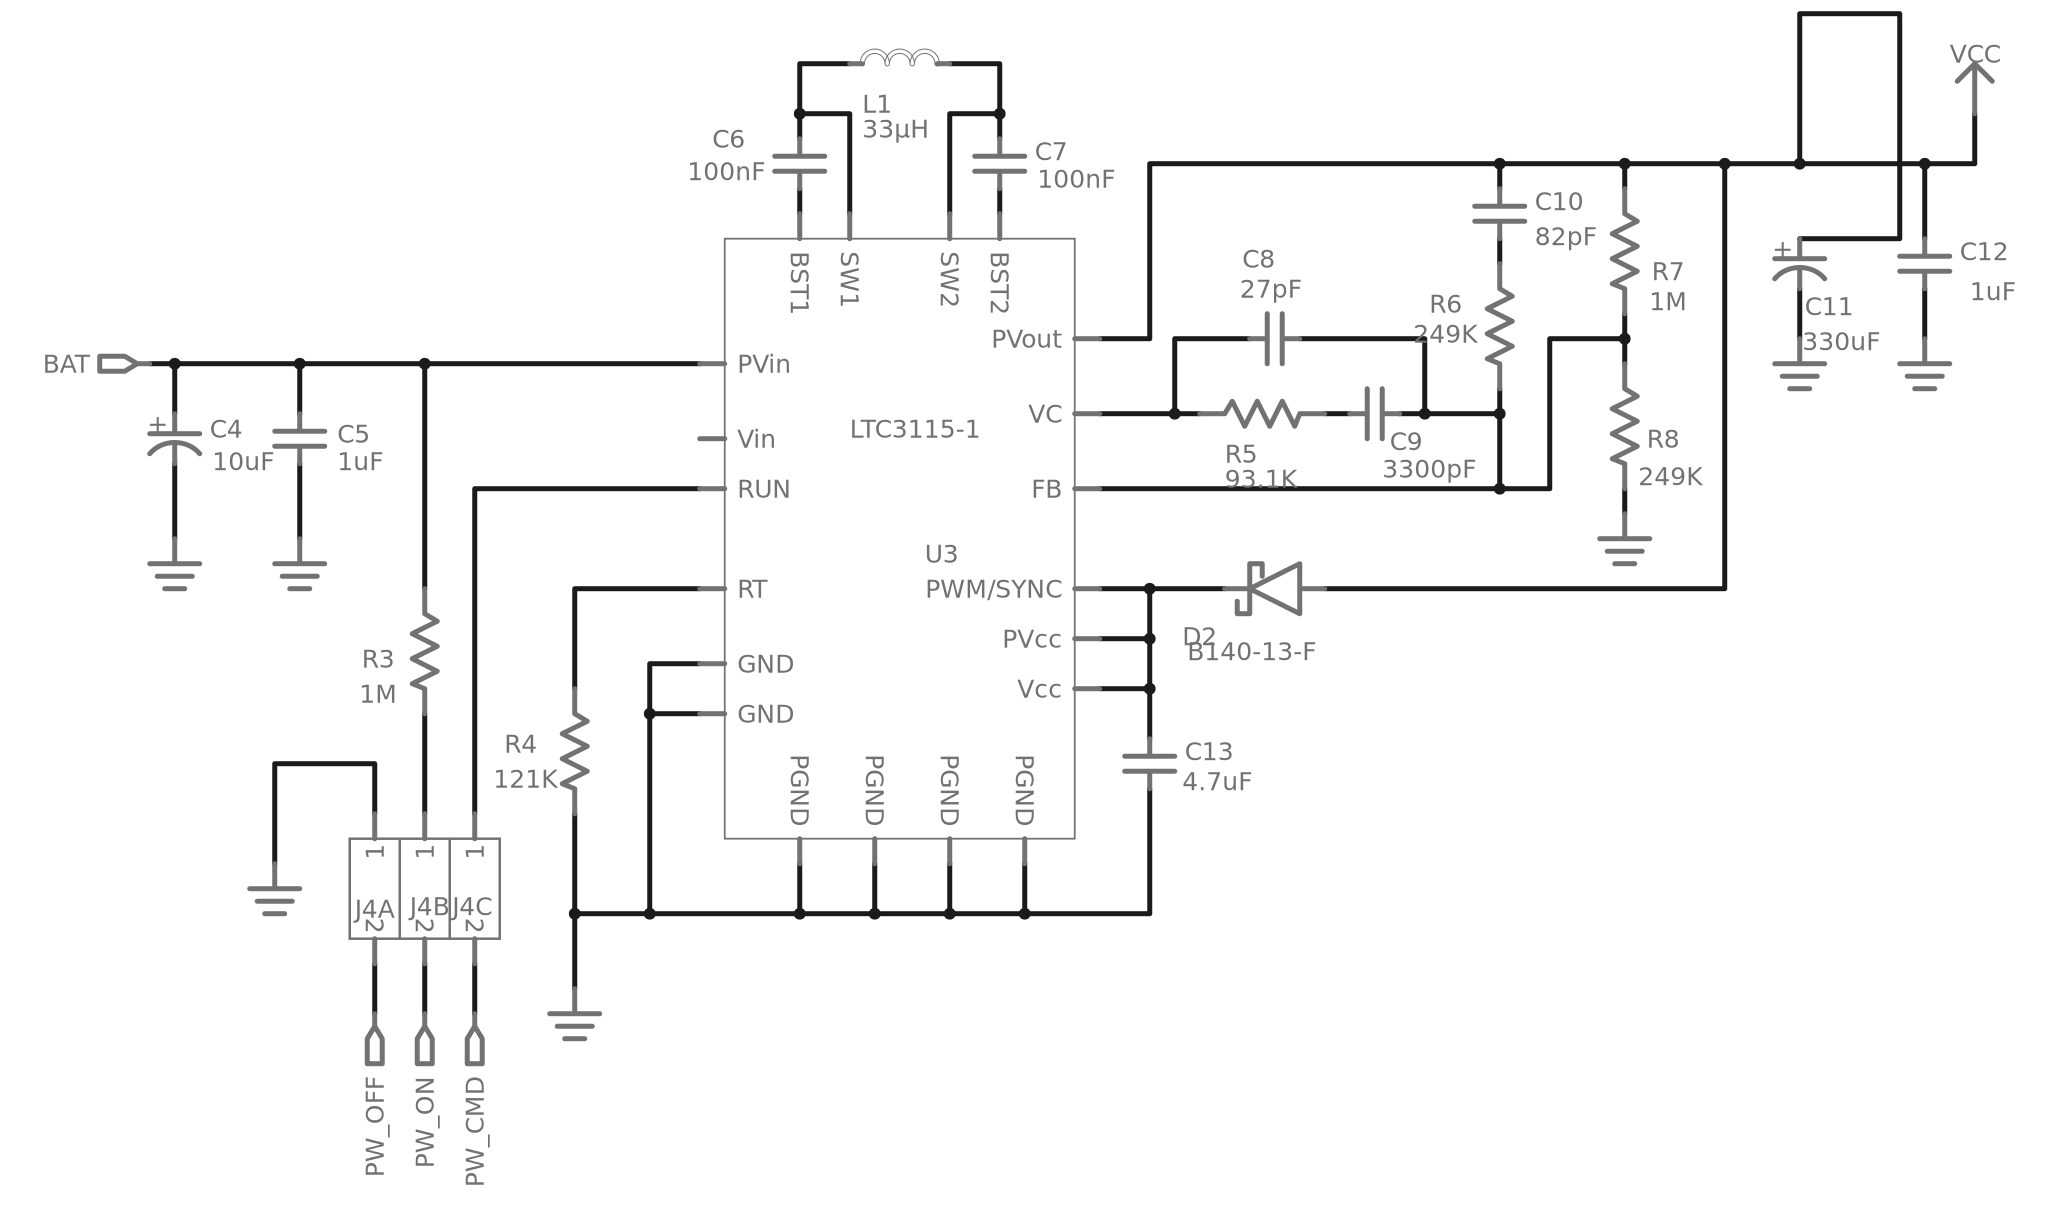
\includegraphics[width=0.85\textwidth,fbox]{img/ElecSch_BuckBoost}
    }
    \caption{Schéma structurel du régulateur de tension}
    \label{ElecSch_BuckBoost}
\end{figure}

    La fonction électronique \emph{régulateur de tension} est réalisée autour du composant LTC3115-1 (repère typographique $U_3$ de la Figure \ref{ElecSch_BuckBoost}).
    Pour rappel, la fonction régulateur de tension a pour rôle de prendre la tension délivrée par la batterie qui varie entre 3.7V et 4.2V suivant sa charge et de la convertir en 5V stabilisé afin d'alimenter le Raspberry Pi, l'amplificateur audio et le driver de led.
    Ce convertisseur de tension est une alimentation à découpage de type Buck-Boost.
    
    La boucle de retour est un filtre du troisième ordre dont la fonction de transfert :
    
    \todo[inline]{TODO}

\begin{figure}[H]
    \centerline{
        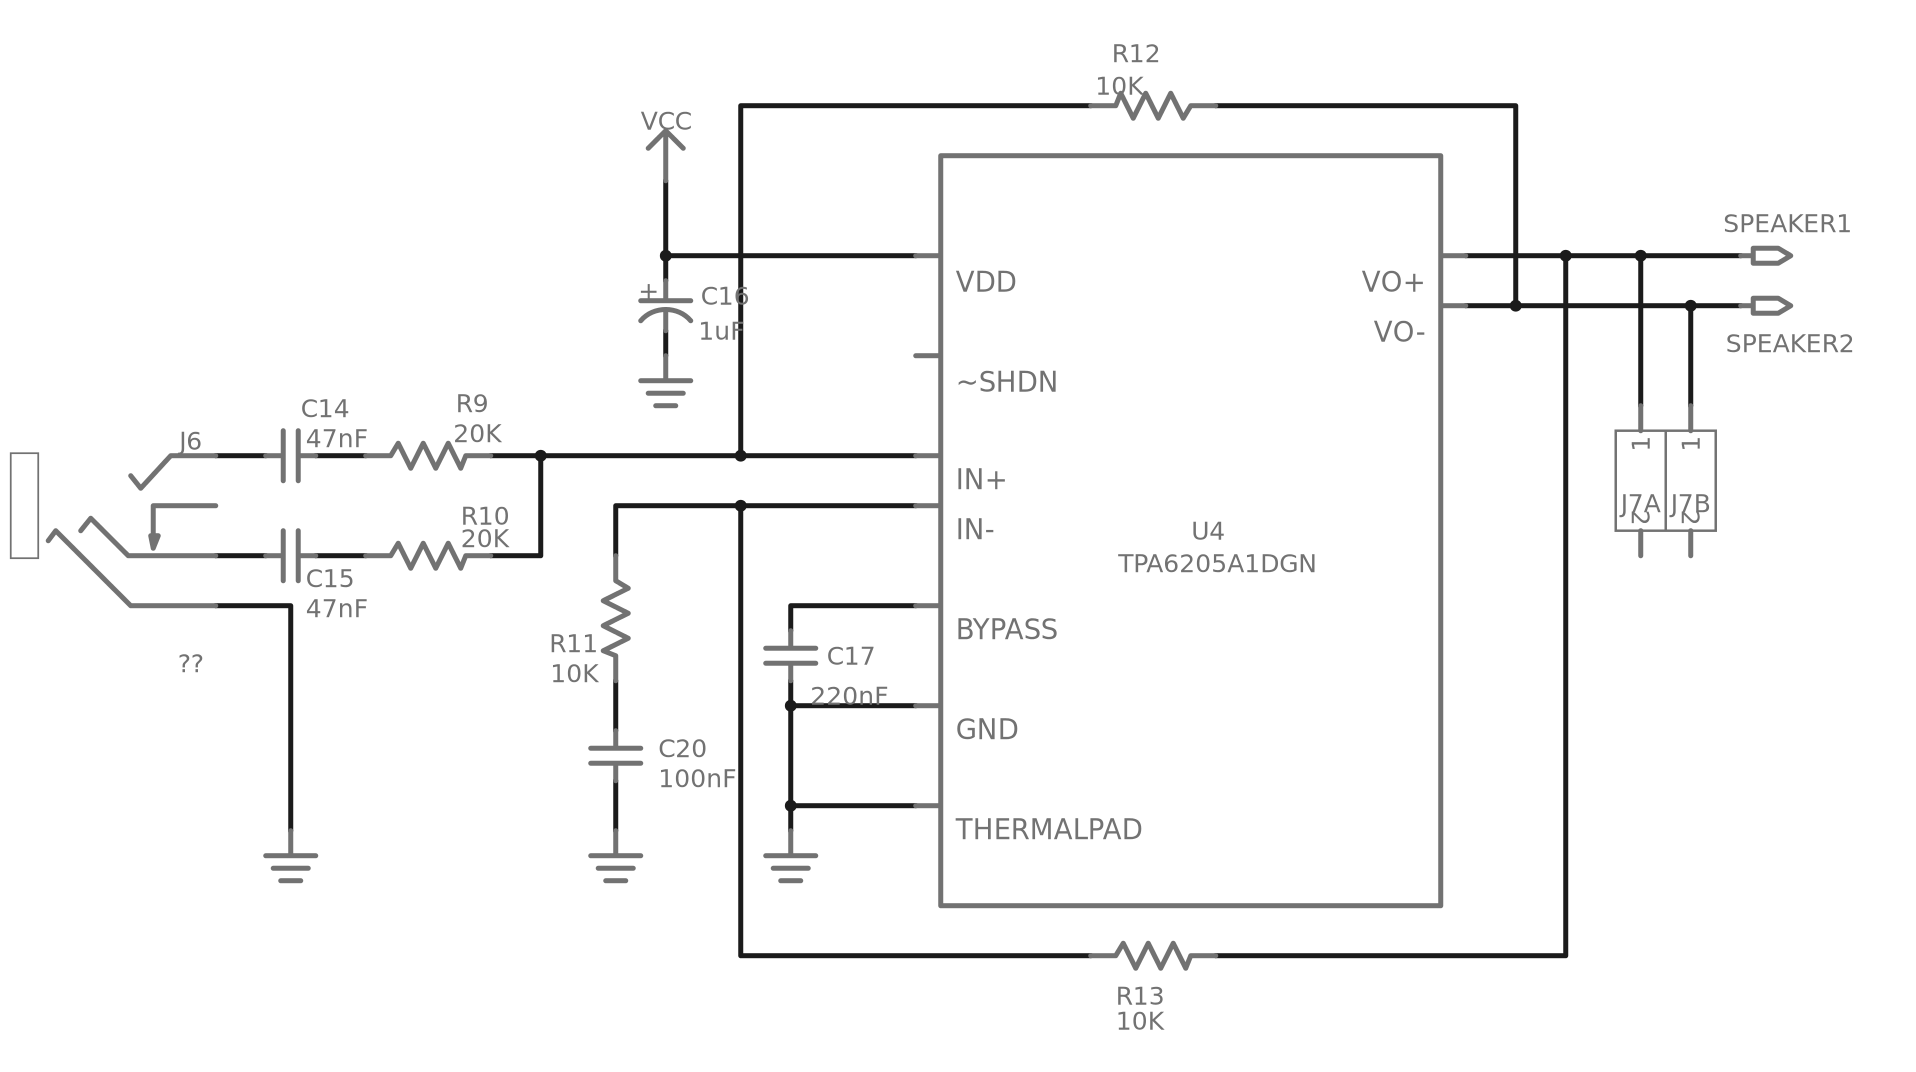
\includegraphics[width=0.85\textwidth,fbox]{img/ElecSch_AudioAmp}
    }
    \caption{Schéma structurel de l'amplificateur audio}
    \label{ElecSch_AudioAmp}
\end{figure}

    La fonction électronique \emph{amplificateur audio} est réalisée autour du composant TPA6205A1DGN (repère typographique $U_4$ de la Figure \ref{ElecSch_AudioAmp}).
    Pour rappel, la fonction amplificateur audio a pour rôle de récupérer le signal audio stéréo de synthèse vocale généré par le Raspberry Pi disponible sur le connecteur jack 3.5 mm, de sommer les deux voies et d'amplifier le signal afin d'attaquer le haut-parleur de 8 $\Omega$ relié au bornier $J_7$.
    
    Les deux condensateurs $C_{14}$ \& $C_{15}$ sont des condensateurs de liaison permettant d'enlever la composante continue de chaque voie.
    Les impédances de chaque entrée différentielle de l'amplificateur doivent être équilibrées, pour cela il faut respecter les relations suivantes :
    
\begin{subequations}
\begin{align}
C20 &= C15 + C14 \\
100nF &\approx 47 nF + 47 nF
\end{align}
\end{subequations}
\begin{subequations}
\begin{align}
R_{11} &= \frac{R_9 \times R_{10}}{R_9 + R_{10}}\\
10 k\Omega &= \frac{(20 k\Omega)^{2}}{2 \times 20 k\Omega}
\end{align}
\end{subequations}
    
    Le gain d'amplification et la fréquence de coupure pour chaque voix est :
    
\begin{equation}
Gain = 20 \times log \left (\frac{2 \times 150 k\Omega}{R_9}\right ) = 20 \times log \left (\frac{2 \times 150 k\Omega}{R_{10}}\right ) \approx 23.5 dB
\end{equation}
\begin{equation}
F_{C} = \frac{1}{2 \pi R_9 C_{14}} = \frac{1}{2 \pi R_{10} C_{15}} = 169 Hz
\end{equation}

\begin{figure}[H]
    \centerline{
        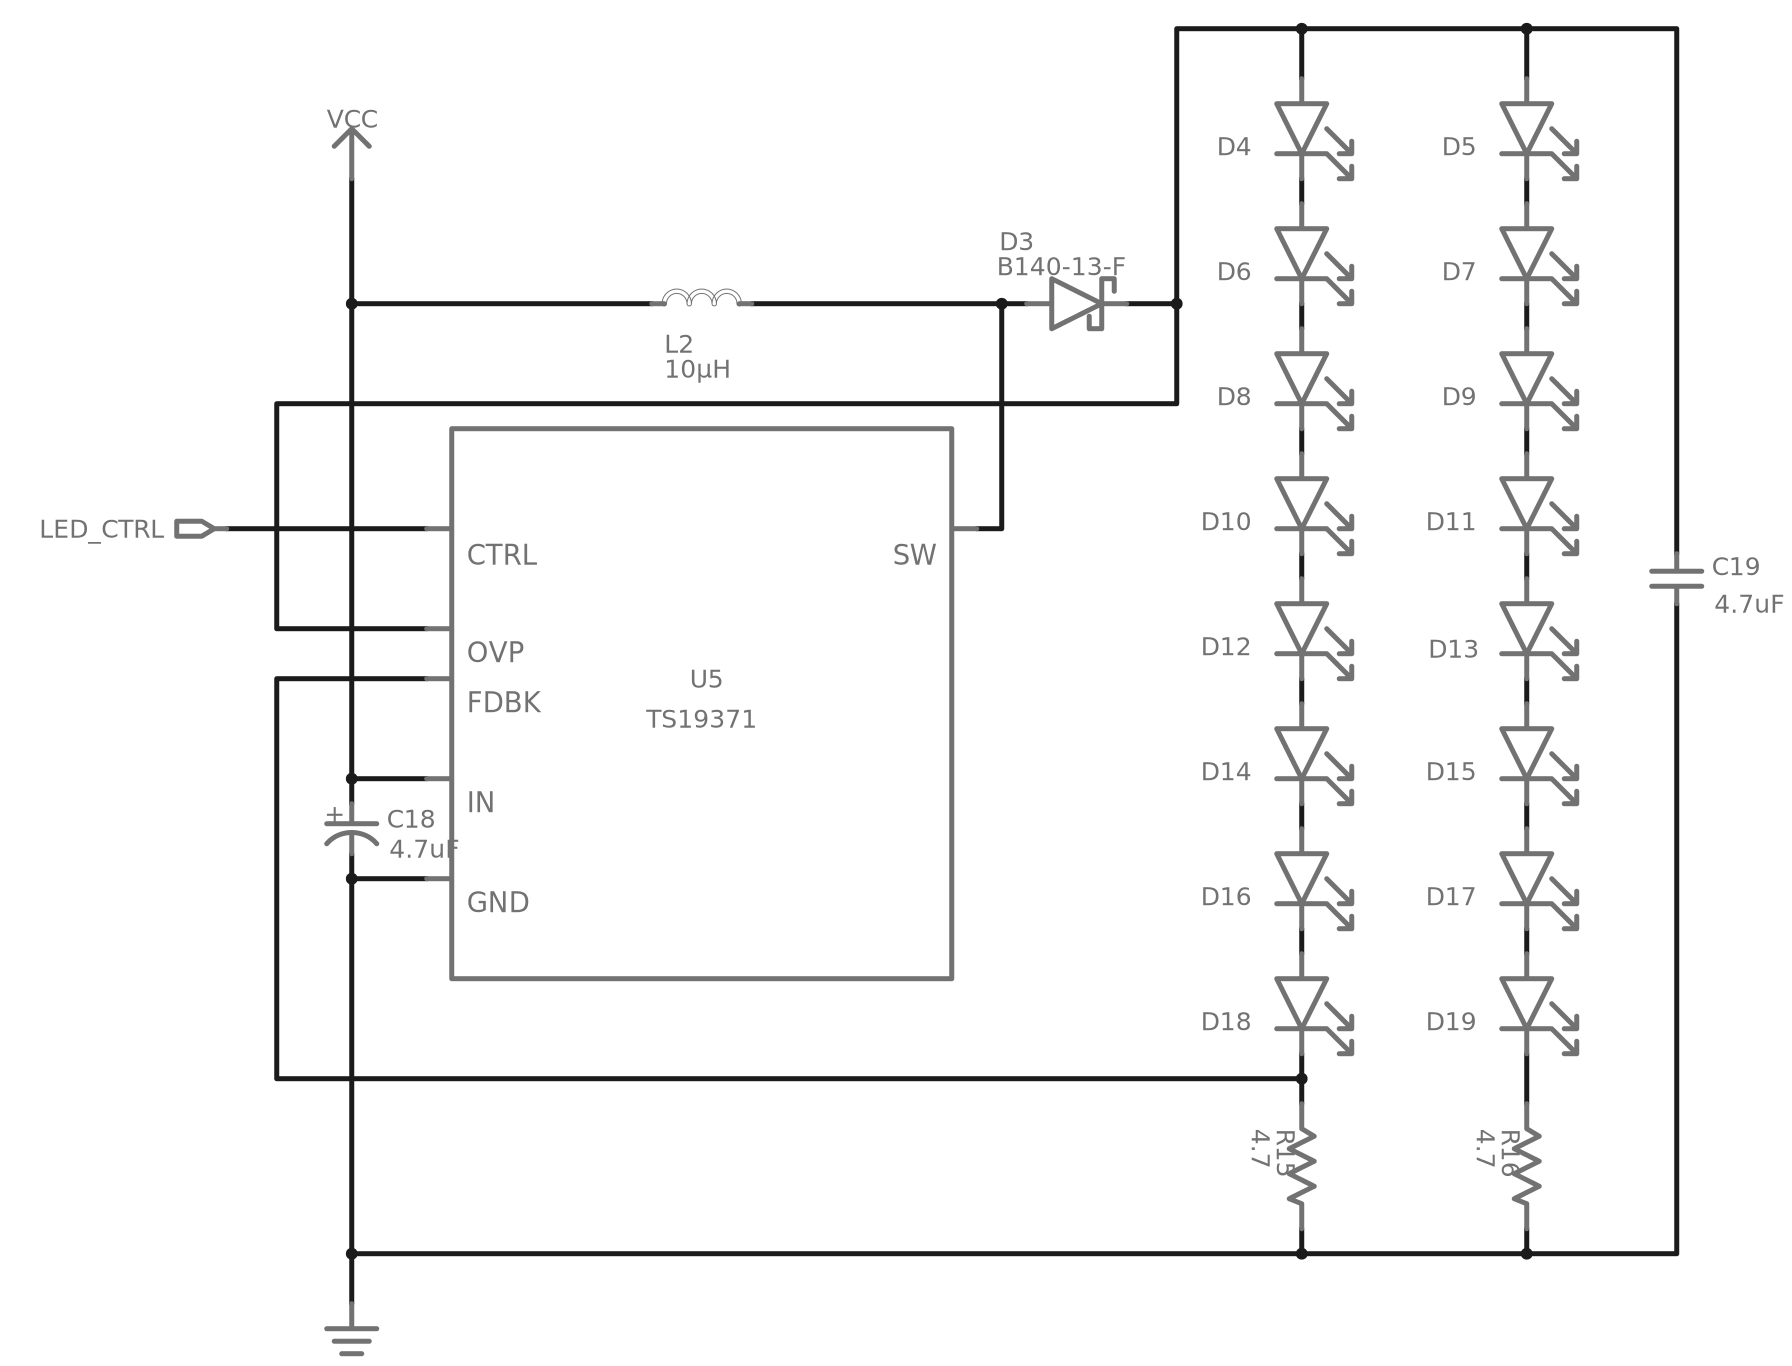
\includegraphics[width=0.85\textwidth,fbox]{img/ElecSch_LedDriver}
    }
    \caption{Schéma structurel de l'éclairage}
    \label{ElecSch_LedDriver}
\end{figure}

    La fonction électronique \emph{d'éclairage} est réalisée autour du driver de leds TS19371 (repère typographique $U_5$ de la Figure \ref{ElecSch_LedDriver}).
    Pour rappel, la fonction électronique a pour rôle d'alimenter les 16 leds blanches en fonction du signal PWM \emph{LED\_CTRL} délivré par le Raspberry Pi.
    
    Le driver de led permet de piloter deux lignes de 8 leds en série en augmentant la tension d'alimentation $VCC$ de 5V jusqu'à 18V.
    Ceci se fait en asservissant le courant sur chacune des deux lignes.
    La valeur du courant est fixée par le choix de $R_{15}$ et de $R_{16}$ :
    
\begin{equation}
R_{15} = R_{16} = \frac{95 mV}{I_{LED}} = \frac{95 mV}{20 mA} \approx 4.7 \Omega
\end{equation}

\begin{figure}[H]
    \centerline{
        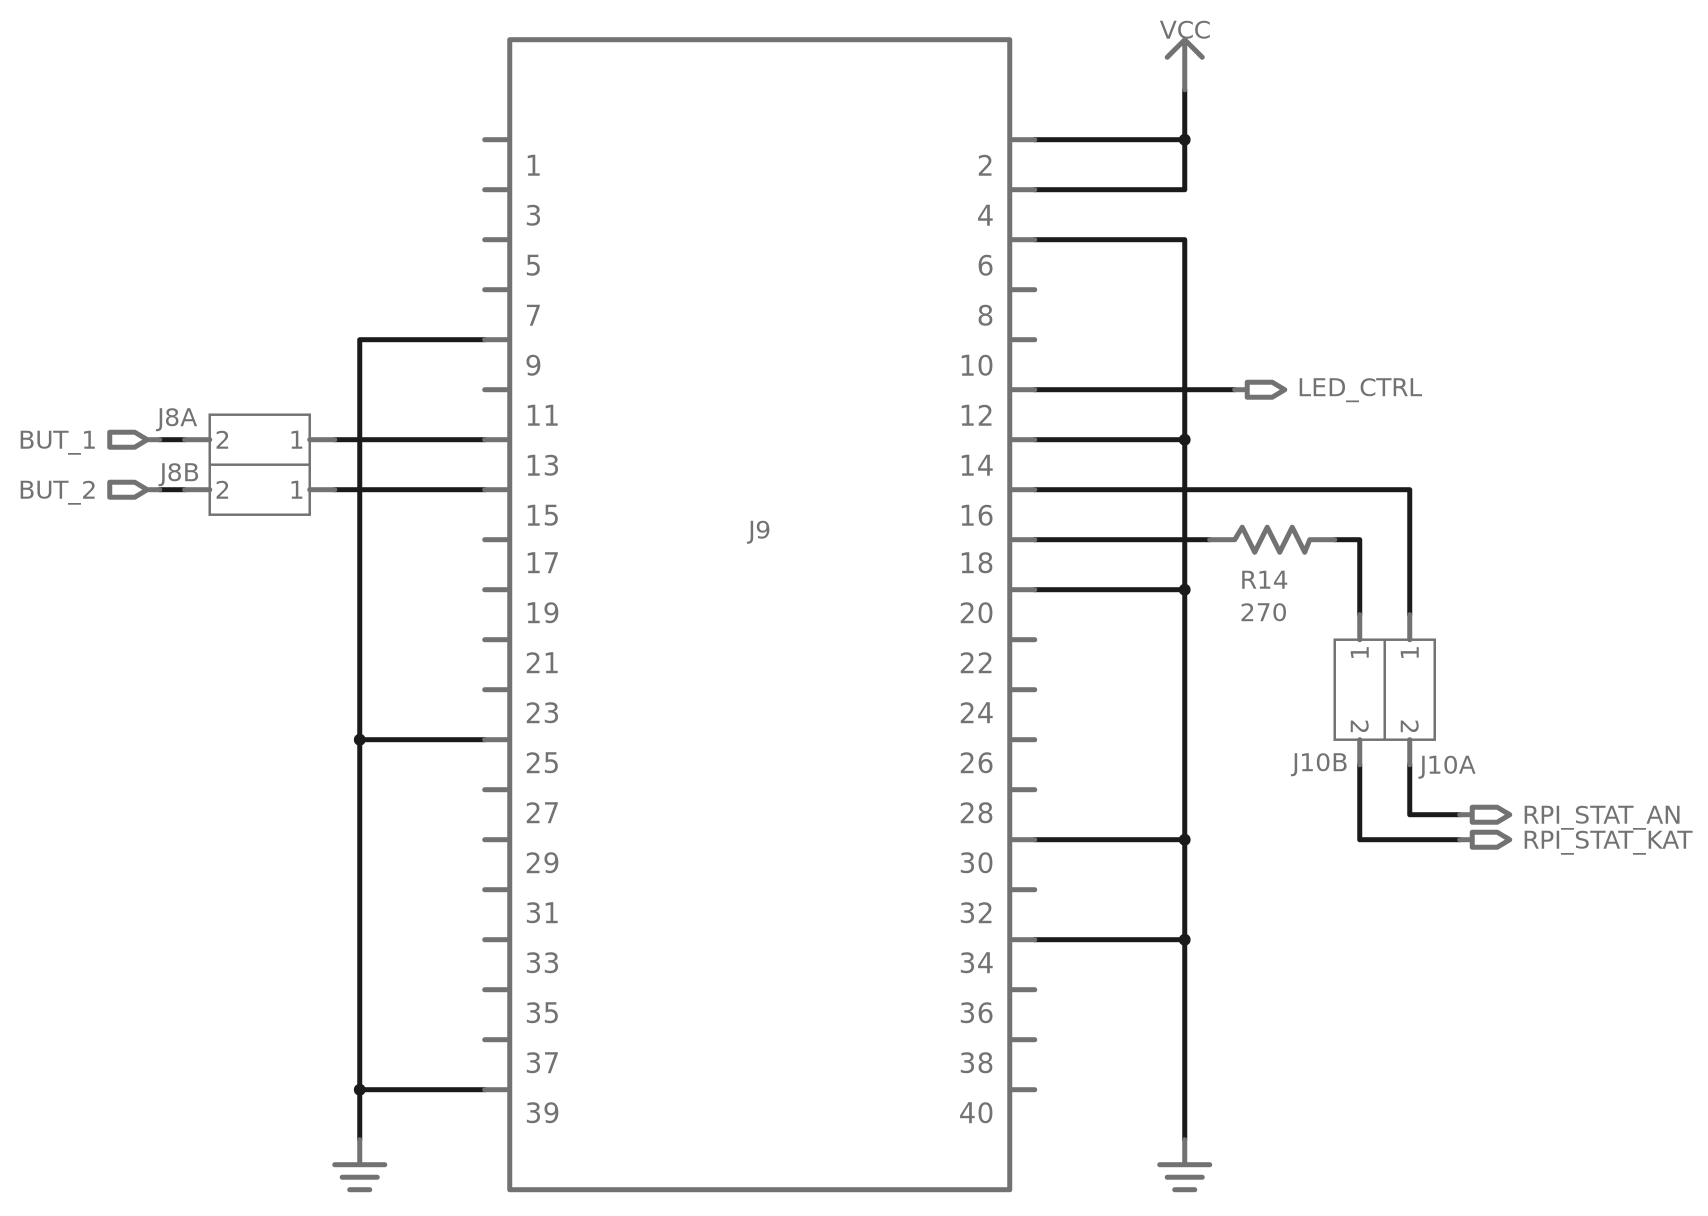
\includegraphics[width=0.85\textwidth,fbox]{img/ElecSch_RPiConn}
    }
    \caption{Schéma structurel du connecteur du Raspberry Pi}
    \label{ElecSch_RPiConn}
\end{figure}

Finalement sur la Figure \ref{ElecSch_RPiConn} on retrouve le connecteur de la Raspberry Pi sur lequel est reliée l'alimentation 5V, un premier bornier pour la lecture d'un bouton-poussoir, un second bornier pour le pilotage d'une led et enfin le signal PWM \emph{LED\_CTRL} pour le pilotage de l'éclairage.
    
    \section{Mécanique}
    % parlé fabrication boitier
    Le boitier mécanique a été modélisé sur le logiciel de CAD en ligne OnShape.
    Il est composé de trois pièces imprimées en PLA qui forment un cube d'environ 12 cm de côté.
    Un jeu de 0.2 mm a été prévu entre les pièces pour faciliter l'assemblage.
    L'assemblage final est présenté sur le dessin technique page \pageref{mecdrawing}.
    
    La première pièce constitue la trappe d'accès, elle forme une des faces du cube.
    Elle est maintenue aux deux autres pièces à l'aide de quatre vis M3 à tête conique afin d'en permettre le démontage/remontage ainsi que l'accès aux composants.
    Sur sa face sont percés les évents du haut-parleur, ce dernier est maintenu à l'aide de deux rails, ce qui permet un montage sans visserie ni colle.
    Le compartiment pour la batterie a été placé sur cette pièce.
    Les trois perçages visibles ont été placés afin d'y accueillir deux leds, l'une sert d'indicateur de charge de batterie et l'autre d'indicateur de statut du Raspberry Pi, ainsi qu'un bouton-poussoir pour lancer un scénario de reconnaissance.
    
    
    \includepdf[pages={-},angle=90]{img/Drawing_Boitier.pdf}
    \label{mecdrawing}
    
    \section{Webservices}
    
    L'ensemble des Webservices tels qu'ils sont présentés dans l'annexe A de \cite{OBCdS} ont été implémentés avec le framework Scalatra.
    L'ensemble du projet utilise le moteur de production SBT, cet outil permet de gérer notamment les dépendances de librairies, la compilation et le test.
    
    La persistance des données est faite sur une base de données dite NoSQL, MongoDB.
    L'accès à MongoDB en Scala se fait via le driver Casbah, il permet de manipuler les documents MongoDB de la même manière que l'on manipule les collections en Scala.
    Le module GridFS de MongoDB est utilisé afin d'outrepasser la limite des 16 Mo par fichier.
    
    Les services qui font appel soit à des ressources matérielles de la Raspberry Pi, soit à des tâches de calcul intensives --- comme le traitement d'image et la classification automatique --- le font en faisant des commandes système.
    Les programmes qui sont appelés ont été écrits en C++.
    
    
    % Stack scalatra + mongodb + call to external program (native c++ opencv) pico2wave => les webservices
    